\section{.................} 

\textbf{}\\


\begin{flushleft}

\begin{center}
	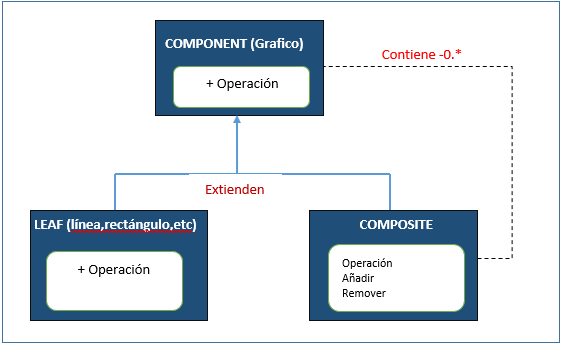
\includegraphics[width=10cm]{./Imagenes/composite1} 
	\end{center}
\begin{itemize}
\textbf{Uso}

\textbf{}\\
\textbf{Aplicación}


Usar el patrón COMPOSITE cuando:


  \item Se quiere representar jerarquías de objetos todo-parte.
  \item Se quiere ser capaz de ignorar la diferencia entre objetos individuales y composiciones de objetos.  Los clientes tratarán a todos los objetos de la estructura compuesta uniformemente.

\end{itemize} 

\textbf{}\\
\textbf{}\\
\textbf{}\\
\textbf{}\\
\textbf{}\\
\textbf{}\\
\textbf{Estructura}

\textbf{}\\ 
\textbf{}\\ 

\begin{center}
	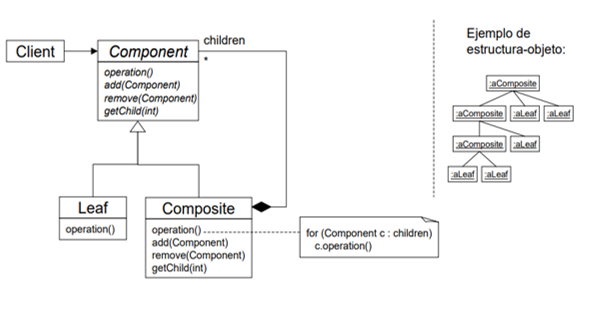
\includegraphics[width=10cm]{./Imagenes/composite2} 
	\end{center}

\textbf{Participantes}

El patrón Composite requiere mínimo de tres componentes para poder existir los cuales son Componente, Leaf o Rama y Composite.

\begin{enumerate}[a)]
        \item \textbf{ Component (Grafico)}
Generalmente es una interface o clase abstracta la cual tiene las operaciones mínimas que serán utilizadas, este componente deberá ser extendido por los otros dos componentes Leaf y Composite. En nuestro ejemplo esto podría representar de forma abstracta un ladrillo o toda la casa (Mas adelante comprenderemos porque)

        \item \textbf{ Leaf o Rama (Línea, Rectángulo, Texto)}
El leaf u hoja representa la parte más simple o pequeña de toda la estructura y este extiende o hereda de Component. En nuestro ejemplo, este representaría un ladrillo de nuestra casa.

	\item \textbf{Composite (Dibujo)}
Aquí es donde está la magia de este patrón, ya que el composite es una estructura conformada por otros Composite y Leaf, los Composite tiene los métodos add  (añadir) y remove (remover) los cuales nos permiten agregar objetos de tipo Component, Sin embargo, el Componente es por lo general un Interface o Clase abstracta  por lo que se puede agregar objetos de tipo Composite o Leaf.   Desde el punto de vista del ejemplo de la casa el Composite podría representar un conjunto de ladrillos o la casa completa, Esto desde luego sería agregando varias Ladrillo(Leaf) al Composite para crear una Pared.

	\item \textbf{ Client}
Es la entidad que hará uso del objeto compuesto.
    \end{enumerate}

\textbf{}\\ 
\textbf{}\\ 
\textbf{}\\ 
\textbf{}\\ 
\textbf{}\\ 
\textbf{}\\ 
\textbf{}\\ 
\textbf{}\\ 
\textbf{}\\ 
\textbf{EJEMPLO DE ESTUDIO DEL PATRON COMPOSITE}
Imaginemos un sistema de puntos de venta, en el cual se le pueden vender al cliente una serie de productos, estos productos pueden ser productos simples (Leaf) o paquetes (Composite).  El sistema permitirá crear “Ordenes de Ventas”, las cuales están compuestas por 1 o muchos productos.

\begin{center}
	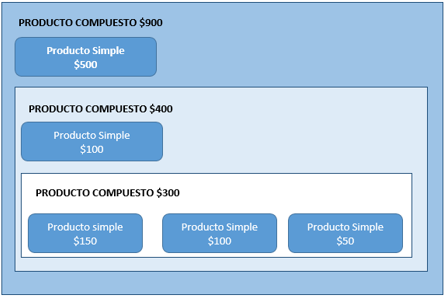
\includegraphics[width=10cm]{./Imagenes/composite3} 
	\end{center}

En la imagen se muestra de forma gráfica cómo está compuesto un paquete.  Los paquetes están creados a partir de un conjunto de productos simples y otros paquetes por lo que el precio de un paquete está calculado por el precio de sus hijos de forma recursiva.  Muestra la estructura de una forma conceptual, sin embargo, la estructura es un poco más compleja, ya que está formado por una estructura de dato llamado “Arbol”

\begin{center}
	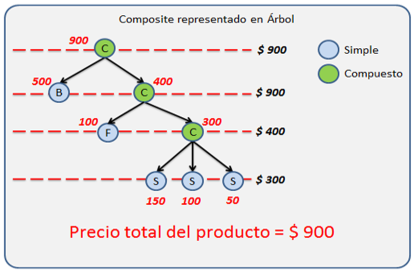
\includegraphics[width=10cm]{./Imagenes/composite4} 
	\end{center}

Esta imagen muestra un solo paquete, está formado de otros productos, simples y compuestos, un compuesto sería otro paquete, el cual tiene dentro más productos simples y como se vio en la figura anterior, el precio de un paquete es calculado por el precio de todos los hijos de forma recursiva.

\textbf{}\\ 
\textbf{}\\
\textbf{}\\
\textbf{}\\
\textbf{}\\
\textbf{}\\

\textbf{CONCLUSION}

\begin{itemize}
\item Define jerarquías de clases hechas de objetos simples y compuestos. 
\item Si el código cliente espera un objeto simple, puede recibir también uno compuesto 
\item Puede hacer el diseño demasiado general. Es complicado restringir el tipo de componentes de un composite.
\item Un paquete es producto compuesto de varios productos simples y otros paquetes.
\item Simplifica el cliente.  Los paquetes y productos simples deberán ser tratados de la misma forma, por lo que deberán tener un padre en común.
\item El precio de un paquete es la suma de todos los productos simples que contenga.
\item El sistema deberá mostrar el total de la Orden y los productos que contiene.
\item Facilita la incorporación de nuevos tipos de componentes


\end{itemize} 





\end{flushleft}